\section{Calibration using a photometric correction {\color{blue} Laurence} }
\label{se:photocorr_calibration}

As discussed in Sect.~\ref{se:obsdate_variations}, observations during the
afternoon sessions or
%the morning session after observations close to the direction of the
%Sun
during sunrise
are deeply affected by the telescope-driven beam
size variations, which are either due to an increase of the main dish
temperature (afternoons) or to a focus drift (sunrises).
For the baseline calibration presented in
Sect.~\ref{se:baseline_calibration}, this effect was mitigated by
discarding the scans acquired during these periods, as defined by the
baseline selection of Sect.~\ref{se:data_selection}. However, in
this section, we address the issue of calibrating in
telescope-driven unstable observing conditions. We discuss a
calibration method that relies on a photometric correction
depending on the beam size. 

When using the photometric correction, no scan selection based on the
observation date is performed. However, the scans from which the
absolute calibration is derived, are selected on the FWHM estimate
using the same criteria as for the baseline calibration. Thus, only
the scans that are moderately affected by the beam effect are included
in the absolute calibration in order not to include twice the
photometric correction uncertainties in the error budget (once for the
absolute calibration and once for the photometry).


\subsection{Photometric correction methods}
\label{se:photocorr_methods}

When the beam size broaden due to e.g. temperature increase of the
telescope main dish, the flux density is smeared in a larger solid angle and
the flux density estimator, which is based on the amplitude fit of a
Gaussian beam of fixed FWHM as described in
Sect.~\ref{se:flux_density_equation}, is biased toward low flux densities.

Considering only the main beam broadening, modeled as a Gaussian of
size $FWHM' = 2 \sqrt{2\ln{2}} \, \sigma '$, we show in
Sect.~\ref{se:photometric_correction} that
the flux density estimator depends on the size of the convolution
function between the enlarged $\sigma '$ Gaussian and the 
$\sigma_0$ fixed width Gaussian of our reference system.
A corrected flux density estimator $\hat{S}_{pc}$ can be derived from
the uncorrected estimator as
\begin{equation}
  \hat{S}_{pc} = f(\sigma')\hat{S},  
\end{equation} 
where the photometric correction $f$ reads
\begin{equation}
  f(\sigma') = \frac{(\sigma'^2 + \sigma_0^2)}{2 \sigma_0^2}. 
\end{equation} 

The photometric correction relies on the measure of the current beam
size $\sigma ’$. The induced uncertitude on the flux density
measurments depends on the precision of which we are able to monitor
the beam size. 

We perform two case studies: Sect.~\ref{se:photocorr_demo} presents a demonstration
calibration assuming the beam is precisely monitored, whereas
Sect.~\ref{se:photocorr_pointing} addresses a practical calibration relying
on a beam monitoring using pointing scans. 

\subsubsection{Demonstration case}
\label{se:photocorr_demo}

For the demonstration case, shortened as 'demo' hereafter, we use a
photometric correction based on the Gaussian FWHM fitted on the map
of the source. This method thus applies only on point-like
sources that are bright enough for an accurate fit of the beam to be
obtained using a single scan.  

The beam size is estimated by fitting a 2D Gaussian from the map and
forming the geometrical $\sigma$, $\sigma_{\rm{geom}} = (\sigma_x^2 +
\sigma_y^2)^{1/2}$.  

This yields a slightly biased estimator of the beam variation since
$\sigma_{\rm geom}$ slightly depends on the flux of the source. The 2D
Gaussian fit yields slightly broaden $\sigma_{\rm{geom}}$ for bright
sources (e.g. planets) to accomodate for the side lobes, which are
measured with high signal-to-noise. We account for the side lobes
impact by correcting $\sigma_{\rm{geom}}$ by a small offset
$\delta_{\rm{sl}}$.





\subsubsection{Practical case using pointing scans}
\label{se:photocorr_pointing}

\addparag{ pointing-based photometric correction}




\subsection{Stability against observing conditions}


\begin{figure}[ht!]
\begin{center}
  % corrected skydip
  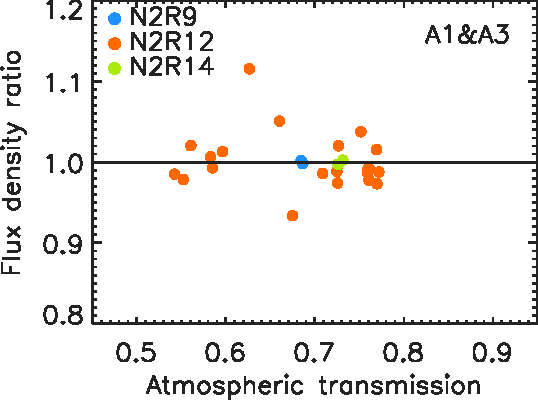
\includegraphics[clip=true, trim={0, -0.3cm, -0.3cm, 0}, width=0.35\textwidth]{Figures/Calibration/plot_flux_density_ratio_obstau_uranus_corrected_skydip_narrow_1mm.pdf}
  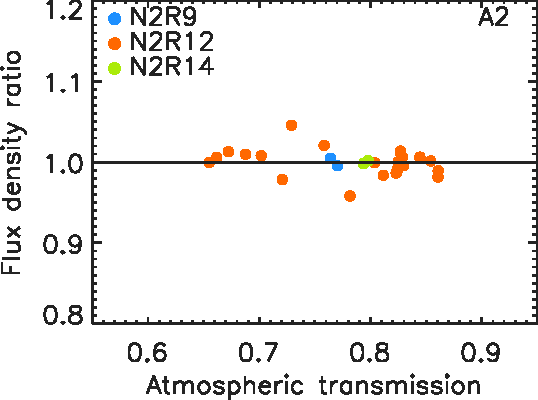
\includegraphics[clip=true, trim={0, -0.3cm, -0.3cm, 0}, width=0.35\textwidth]{Figures/Calibration/plot_flux_density_ratio_obstau_uranus_corrected_skydip_narrow_a2.pdf}
  % taumeter
  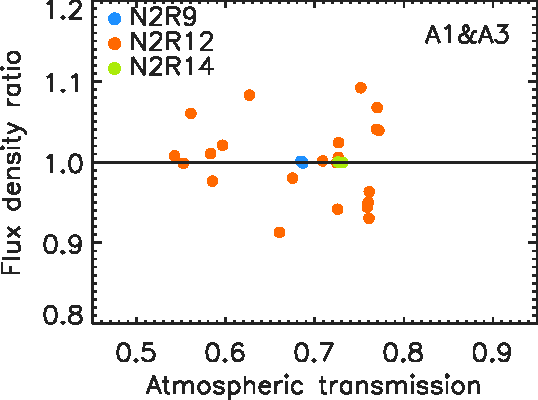
\includegraphics[clip=true, trim={0, -0.3cm, -0.3cm, 0}, width=0.35\textwidth]{Figures/Calibration/plot_flux_density_ratio_obstau_uranus_tau225_narrow_1mm.pdf}
  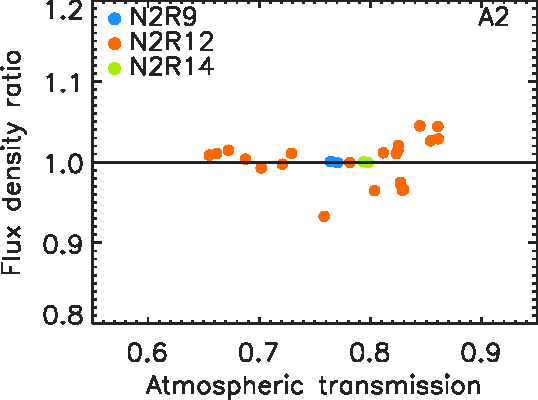
\includegraphics[clip=true, trim={0, -0.3cm, -0.3cm, 0}, width=0.35\textwidth]{Figures/Calibration/plot_flux_density_ratio_obstau_uranus_tau225_narrow_a2.pdf}
  % skydip
  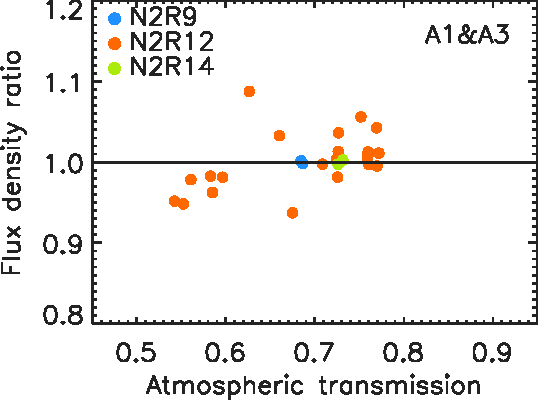
\includegraphics[clip=true, trim={0, -0.3cm, -0.3cm, 0}, width=0.35\textwidth]{Figures/Calibration/plot_flux_density_ratio_obstau_uranus_skydip_narrow_1mm.pdf}
  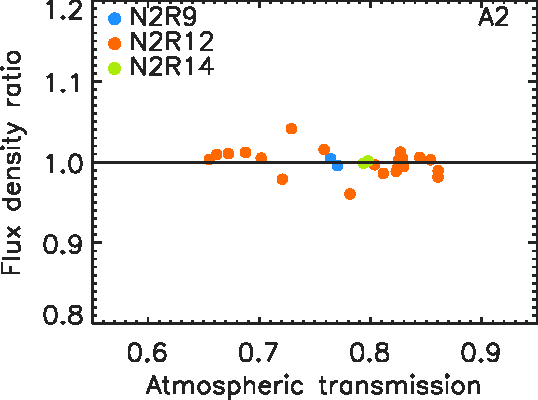
\includegraphics[clip=true, trim={0, -0.3cm, -0.3cm, 0}, width=0.35\textwidth]{Figures/Calibration/plot_flux_density_ratio_obstau_uranus_skydip_narrow_a2.pdf}
  % corr. sky. photocorr demo
  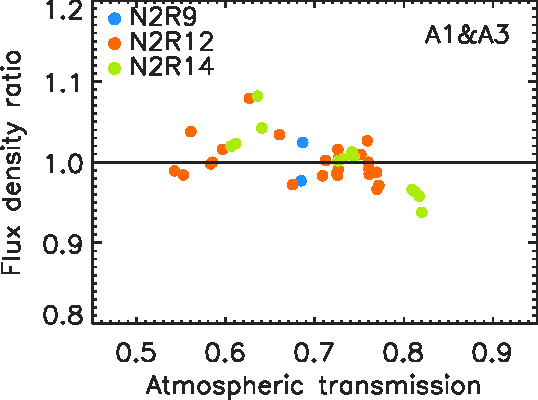
\includegraphics[clip=true, trim={0, -0.3cm, -0.3cm, 0}, width=0.35\textwidth]{Figures/Calibration/plot_flux_density_ratio_obstau_uranus_corrected_skydip_photocorr_demo_narrow_1mm.pdf}
  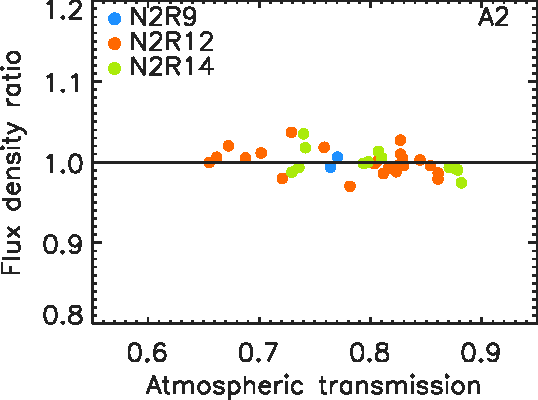
\includegraphics[clip=true, trim={0, -0.3cm, -0.3cm, 0}, width=0.35\textwidth]{Figures/Calibration/plot_flux_density_ratio_obstau_uranus_corrected_skydip_photocorr_demo_narrow_a2.pdf}
  % corr. sky. photocorr pointing
  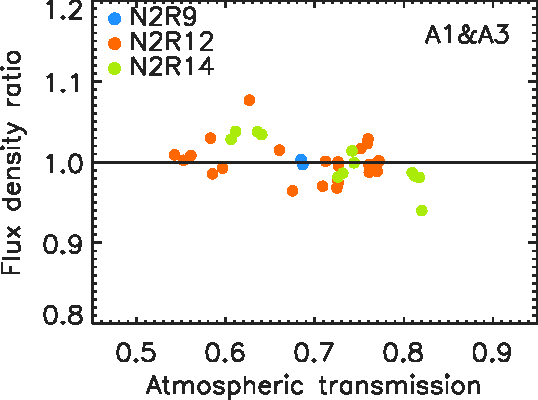
\includegraphics[clip=true, trim={0, -0.3cm, -0.3cm, 0}, width=0.35\textwidth]{Figures/Calibration/plot_flux_density_ratio_obstau_uranus_corrected_skydip_photocorr_pointing_narrow_1mm.pdf}
  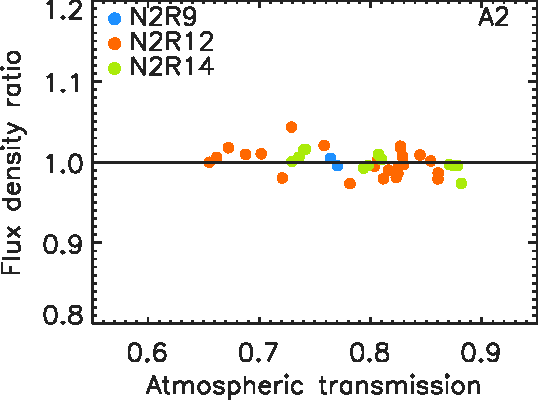
\includegraphics[clip=true, trim={0, -0.3cm, -0.3cm, 0}, width=0.35\textwidth]{Figures/Calibration/plot_flux_density_ratio_obstau_uranus_corrected_skydip_photocorr_pointing_narrow_a2.pdf}
  \caption[Uranus flux density stability against atmospheric
    transmission]{Uranus flux density ratio vs atmospheric transmission
    shown for the $1$-mm array
    combination (left column) and for array 2 (right column) after absolute
    calibration using (\emph{first row}:) the baseline method, as
    well as (\emph{second row}:) the 'taumeter'-based and
    (\emph{third row}:) the 'skydip'-based methods, and methods
    relying to (\emph{fourth row}:) the 'demo' and (\emph{fifth
      row}:) the 'pointing' photometric corrections. These plots
    include all Uranus scans acquired during N2R9, N2R12 and N2R14
    campaigns. }
  \label{fig:calib_uranus_vs_atmtrans_all}
\end{center}
\end{figure}



% ALL METHOD RESULTS 
\begin{table}[th]
\begin{center}
\begin{tabular}{|c|l|c|c|c|c|c|}
  \hline
  \multicolumn{2}{|c|}{}  &  \multicolumn{5}{|c|}{Methods} \\\cline{3-7}
  \multicolumn{2}{|c|}{Characteristics} &  baseline  & taumeter  &  skydip  &  photocorr demo & photocorr pointing \\
  \hline\hline
   \multicolumn{2}{|c|}{$\#$ selected scans} & 26    &       26  &    26    &    38           &    38 \\ 
  \hline 
  Factor &  A1          &   1.00  &  0.97   &  1.13    &   1.02    &   1.01  \\
       &  A3            &   1.00  &  0.97   &  1.02    &   1.02    &   1.00  \\
       &  1mm           &   1.00  &  0.95   &  1.06    &   1.02    &   1.01  \\
       &  2mm           &   1.00  &  0.94   &  0.99    &   1.03    &   1.02  \\
  \hline
  RMS  &  A1            &  3.1    &   4.2   &   3.4    &    3.0    &   2.8 \\
       &  A3            &  3.7    &   4.3   &   3.3    &    3.1    &   2.9 \\
       &  1mm           &  3.2    &   4.5   &   3.3    &    2.7    &   2.5 \\
       &  2mm           &  1.6    &   2.6   &   1.5    &    1.3    &   1.5 \\
\hline\hline
\end{tabular}
\caption[Comparison of calibration results using five methods]{Comparison of calibration results using five methods}
\label{tab:Abs_calibration_results_all}
\end{center}
\end{table}





